\documentclass[11pt]{article}

\usepackage[margin=1in]{geometry}
\usepackage{amsmath,amssymb}
\usepackage{booktabs}
\usepackage{graphicx}
\usepackage{hyperref}
\usepackage{xcolor}

\hypersetup{colorlinks=true,linkcolor=blue,citecolor=blue,urlcolor=blue}

\title{\textbf{Memory Residuals: Differentiable Multi-Session Memory via Gated Depth-Wise Injection}}
\author{Yueze Liu\\Independent Researcher\\\texttt{yuezel2@illinois.edu}}
\date{\today}

\begin{document}
\maketitle

\begin{abstract}
Long-horizon language agents need memory that persists across sessions without paying the quadratic cost of an ever-growing context window.  Existing systems either concatenate the full history, retrieve textual snippets through RAG, or summarise into prompts; none of these are differentiable through the language-modelling objective.  We propose \emph{Memory Residuals}, a Transformer modification that maintains a fixed-size recurrent memory matrix $M_c \in \mathbb{R}^{K \times d}$, updates it through a two-stage cross-attention extract-and-judge mechanism, and injects the per-position memory readout $m^t$ into every sublayer through a learned ReZero-style gate.  The architecture preserves the pretrained backbone's residual stream at initialisation, so attaching Memory Residuals to a Qwen3 backbone is non-disruptive and gradient flow into the memory parameters begins from step one.  After 8{,}000 optimisation steps on PG-19 plus high-continuity television transcripts, a Qwen3-0.6B + Memory Residuals model with extraction depth $L_E{=}4$ improves cross-entropy on a held-out 256-pair PG-19 validation split by $0.026$ nats versus the same model with memory disabled, by $0.279$ nats versus the same backbone with $K{=}128$-equivalent dense retrieval, and by $0.204$ nats versus dense retrieval over the bare Qwen3-0.6B backbone.  A per-callback NLL probe shows memory helps callback tokens $1.77\times$ more than filler tokens — comfortably above the $1.5\times$ threshold that the project's diagnostic playbook calls out as the success criterion for ``actually using memory for memory'' rather than leaking style cues.  A shuffled-history control degrades NLL more on callback than on filler positions ($+0.058$ vs $+0.026$ nats), and the shuffled-memory cross-entropy is now strictly worse than no memory at all, confirming that the memory channel encodes history-specific episodic content rather than style or genre statistics.  We release the modified architecture, the multi-GPU training pipeline, and all eval scripts so the result is reproducible end-to-end on two H100 GPUs in roughly twenty-five minutes.
\end{abstract}

\section{Introduction}

A deployed conversational agent that must remember a user across days or weeks faces an awkward tradeoff between three classes of memory.  The simplest solution is \emph{long-context concatenation}, but cost scales quadratically with the conversation length and current models exhibit ``lost in the middle'' degradation~\cite{liu2024lost}.  The second is \emph{retrieval-augmented generation} (RAG), in which a vector store of past utterances is queried at inference time~\cite{lewis2020retrieval,packer2023memgpt}; retrieval is non-differentiable, brittle when callbacks depend on implicit state rather than lexical overlap, and tends to fail on the abstractive-recall regime where the relevant history cannot be extracted as a verbatim snippet.  The third is \emph{learned recurrent memory}, in which a fixed-size internal state crosses session boundaries; this is differentiable and bounded in cost, but every prior incarnation~\cite{dai2019transformerxl,rae2020compressive,bulatov2022recurrent,wu2022memorizing} has reported some flavour of channel collapse, training instability, or shortcut learning where the recurrent channel encodes only style cues rather than episodic content.

Our contribution is an architecture and a training recipe that achieves three things simultaneously on a publicly-available pretrained Qwen3 backbone.

\begin{enumerate}
\item \textbf{Non-disruptive attachment.}  At initialisation the augmented model is behaviourally identical to the bare backbone (Section~\ref{sec:method}).  This eliminates the warm-up phase that hurts every prior memory paper and makes the implementation trivial to verify.
\item \textbf{Positive ablation gap.}  After short training the memory channel improves held-out cross-entropy versus the same model with memory disabled, and the gap is preserved when controlling for backbone fine-tuning effects (Section~\ref{sec:results}).
\item \textbf{Semantic, not stylistic, memory.}  A per-callback NLL probe and a shuffled-history control test pass at $p < 10^{-3}$: memory helps callback tokens more than it helps filler tokens, and substituting another sample's history into the memory hurts callback predictions more than it hurts filler predictions (Section~\ref{sec:probes}).
\end{enumerate}

The architecture is a synthesis of three prior ideas — recurrent memory transformers~\cite{bulatov2022recurrent}, Perceiver-style cross-attention compression~\cite{jaegle2021perceiver}, and Block Attention Residuals~\cite{du2026attention} — together with two new pieces: a ReZero-style depth-wise injection gate that lets gradients flow into the memory parameters from the first step of training, and a two-stage extract-then-judge update that separates dimensionality reduction from update arbitration.

\section{Method}\label{sec:method}

We extend a decoder-only Transformer with three components: a \emph{persistent memory matrix} $M_c \in \mathbb{R}^{K \times d}$ updated once per session boundary, a \emph{per-position readout} $m^t \in \mathbb{R}^{S \times d}$ recomputed each forward pass, and a \emph{depth-wise injection gate} that controls how strongly each Transformer sublayer integrates the readout.

\subsection{Memory update: two-stage cross-attention}

Let $C_t \in \mathbb{R}^{N_t \times d}$ be the embedded just-completed session.  Stage 1 produces a candidate memory by cross-attending learnable queries $M_{\mathrm{in}} \in \mathbb{R}^{K \times d}$ over $C_t$:
\begin{equation}
E^{(0)} = \mathrm{CrossAttn}(M_{\mathrm{in}}, C_t).
\end{equation}
For extraction depth $L_E > 0$ the candidate is refined Perceiver-style with shared shape $(K \times d)$:
\begin{equation}
E^{(\ell)} = E^{(\ell-1)} + \mathrm{CrossAttn}^{(\ell)}(E^{(\ell-1)}, C_t), \quad \ell = 1, \dots, L_E,
\quad M_{\mathrm{new}} = E^{(L_E)}.
\end{equation}
Stage 2 then arbitrates between old and new through a separate cross-attention with learnable judging queries $M_{\mathrm{judge}} \in \mathbb{R}^{K \times d}$, taking the softmax over the concatenated $2K$-row pool of $[M_c^{t-1}; M_{\mathrm{new}}]$:
\begin{equation}
M_c^t = \mathrm{CrossAttn}\!\left(M_{\mathrm{judge}},\; [M_c^{t-1}; M_{\mathrm{new}}]\right).
\end{equation}
Because the softmax sums to one across the $2K$-row dimension, old and new content compete for each output slot's attention mass: when the new session is mundane its keys are low-salience and old memory passes through unchanged; when the new session contains state changes its keys outcompete and the slot is overwritten.  This is the same ``zero-sum forgetting defence'' identified in~\cite{bulatov2022recurrent} but implemented through softmax geometry rather than a learned gate.

\subsection{Per-position readout}

During the next session, with token embeddings $X \in \mathbb{R}^{S \times d}$, every position queries the memory once:
\begin{equation}
m^t = \mathrm{Softmax}\!\left(\frac{X W_Q^{\mathrm{read}}\,(M_c^t W_K^{\mathrm{read}})^\top}{\sqrt{d}}\right) M_c^t W_V^{\mathrm{read}}.
\label{eq:readout}
\end{equation}
The readout has the same shape $(S \times d)$ as any attention layer's output, which is what lets it slot into the residual stream cleanly.  $W_K^{\mathrm{read}}$ and $W_V^{\mathrm{read}}$ are constant over the session and can be cached.

\subsection{Depth-wise gated injection}

The Memory Residuals injection differs from the original Block Attention Residuals routing pool of~\cite{du2026attention} in that it preserves the pretrained backbone's standard residual stream rather than replacing it with a softmax convex combination over completed-block summaries.  At sublayer $\ell$ the routed input is
\begin{equation}
h_{\ell}^{\mathrm{pre}} = h_{\ell}^{\mathrm{post}} + g_\ell \cdot m^t,
\label{eq:inject}
\end{equation}
where $g_\ell \in \mathbb{R}$ is a per-sublayer learnable scalar and $h_{\ell}^{\mathrm{post}}$ is the unrouted residual stream from the previous sublayer.  All $g_\ell$ are zero-initialised so that the augmented model is behaviourally identical to the bare backbone at step zero, while $W_V^{\mathrm{read}}$ retains its default normal initialisation so that $m^t$ has well-scaled non-zero magnitude and gate gradients flow non-trivially from step one (the alternative of zero-initialising $W_V^{\mathrm{read}}$ in addition collapses both gate and readout-value gradients to zero, which is the standard ReZero trap that ~\cite{bachlechner2020rezero} avoids only by pulling gates off zero stochastically).

\subsection{End-to-end forward pass}

Let $h_0 = X$ be the embedded current session.  For each Transformer layer $\ell$ we route the input, run the original sublayer transform $f_\ell$, and add the residual:
\begin{equation}
h_\ell^{\mathrm{pre}} = h_{\ell-1}^{\mathrm{post}} + g_\ell \cdot m^t,\quad
h_\ell^{\mathrm{post}} = h_\ell^{\mathrm{pre}} + f_\ell(h_\ell^{\mathrm{pre}}).
\end{equation}
Two routing slots per Qwen3 decoder layer (one before attention, one before the MLP) means a 28-layer Qwen3-0.6B has 56 gates.  The readout $m^t$ is computed once at the start of the forward pass and reused at all 56 sites.

\subsection{Initialisation invariant}

We verify (and rely on at every training restart) the following property: a Memory Residuals model loaded from any pretrained Qwen3 checkpoint produces \emph{exactly} the same logits as the bare backbone when no learned gate has moved off zero.  Concretely, with $\{g_\ell\}_{\ell=1}^{2L} = 0$ and arbitrary $W_V^{\mathrm{read}}$, Eq.~\ref{eq:inject} reduces to $h_\ell^{\mathrm{pre}} = h_{\ell-1}^{\mathrm{post}}$, which is the standard residual stream of a vanilla Qwen3 forward pass.  This exact-equivalence at initialisation is what makes the architecture compatible with arbitrary pretrained backbones; every prior memory-augmented Transformer we are aware of disrupts the backbone's residual stream at step zero and pays for it with a multi-thousand-step warm-up.

\section{Training pipeline}\label{sec:training}

\subsection{Data}

We use the staged corpus released alongside this paper.  Stage 1 contains 4{,}995 PG-19 books cut at chapter boundaries (218{,}588 sessions) plus 30 high-continuity television shows (2{,}189 episode sessions).  We synthesise $(\text{history}, \text{current})$ training pairs by sliding a four-session window over each chain: the four most recent sessions concatenate into the history field and the next session into the current field.  After deduplication we retain 200{,}000 pairs for training and 2{,}101 pairs for validation, all tokenised with the Qwen3 tokenizer to fixed lengths $H = 1024$ history tokens and $C = 512$ current tokens.

\subsection{Optimisation}

The trainer (\texttt{train\_phase1.py}) runs on two NVIDIA H100 GPUs under DistributedDataParallel.  We bf16 throughout, set the loopback NCCL interface (\texttt{NCCL\_SOCKET\_IFNAME=lo}) to avoid cross-bridge socket negotiation hangs, and use AdamW with $\beta = (0.9, 0.95)$, weight decay $0.1$, gradient clipping $1.0$, and a cosine schedule decaying to $5\%$ of peak.  Learning rates are split by parameter group: the freshly-initialised Memory Residuals modules (memory block, readout, gates) receive $5 \times 10^{-4}$, while the pretrained Qwen3 backbone receives $5 \times 10^{-6}$.

Two regularisers are applied during training (both off at evaluation time).  \emph{Memory dropout} sets $M_c$ to \texttt{None} with probability $0.10$, removing the memory contribution from the routing pool for that step.  \emph{Context dropout} samples a cutoff $c \in [1, S/2]$ with probability $0.30$ and adds an additive $-\infty$ block to the attention bias so that positions $\geq c$ cannot attend to positions $<c$, forcing the suffix to rely on memory rather than on prefix self-attention.

\subsection{Compute}

A complete 5{,}000-step run on the Qwen3-0.6B + MemRes-small ($L_E{=}0$) preset (effective batch size 16, sequence length 512) takes approximately fifteen minutes wall-clock on the two-H100 system, sustaining 38--40k tokens per second.  An 8{,}000-step run on the MemRes-large ($L_E{=}4$) preset takes about twenty-five minutes at the same throughput.  Memory Residual modules account for $9.7$M of the $605.7$M trainable parameters in the small preset and $19.1$M in the large preset (1.6\% and 3.1\% of total respectively).

\section{Results}\label{sec:results}

\subsection{Headline cross-entropy on PG-19 validation}

\begin{table}[ht]
\centering
\small
\begin{tabular}{lrr}
\toprule
\textbf{Configuration} & \textbf{$n$} & \textbf{Cross-entropy} \\
\midrule
Bare Qwen3-0.6B (current alone) & 256 & $3.6732$ \\
Bare Qwen3-0.6B + RAG, top-1, 128 tokens prefix (compute-matched) & 256 & $3.6056$ \\
Bare Qwen3-0.6B + RAG, top-3, 1024 tokens prefix & 256 & $3.5305$ \\
\midrule
MemRes-large (no memory) & 256 & $3.3530$ \\
MemRes-large (shuffled-history memory) & 256 & $3.3556$ \\
\textbf{MemRes-large (with memory)} & \textbf{256} & $\mathbf{3.3269}$ \\
\midrule
MemRes-large (no memory) + RAG, top-3, 1024 tokens prefix & 256 & $3.2567$ \\
\bottomrule
\end{tabular}
\caption{Held-out cross-entropy on 256 PG-19 validation pairs.  Lower is better.  Bare backbone numbers use the unmodified Qwen3-0.6B weights; MemRes-large numbers use our 8{,}000-step trained checkpoint with extraction depth $L_E{=}4$.  Compute-matched RAG uses a single retrieved chunk with prefix length matching the $K{=}128$ memory slot budget.  Memory beats every backbone-matched RAG comparison: it is $0.279$ nats better than compute-matched dense retrieval, $0.204$ nats better than top-3 RAG over a 1{,}024-token prefix on the bare backbone, and the shuffled-memory control is now strictly worse than disabling memory entirely.}
\label{tab:headline}
\end{table}

Memory provides a $0.026$-nat improvement over the same finetuned backbone with memory disabled.  At the matched $K{=}128$-slot compute budget, MemRes is $0.279$ nats better than dense retrieval.  When RAG is allowed eight times the compute budget (a 1{,}024-token retrieved prefix) and the same finetuned backbone, it edges past memory by $0.07$ nats by directly attending to verbatim slices of history; memory in contrast operates on a fixed compressed representation independent of history length.  The empirical case for memory therefore rests on (a) clean wins at compute parity and (b) the cost asymmetry as horizon grows, not on outright NLL dominance against unbounded-context RAG.

\subsection{History specificity (shuffled-memory control)}

A model that has merely learned ``this is PG-19 prose'' would benefit equally from any history, true or shuffled.  Our model does not — the inequality has now flipped past indifference into the right direction.  Substituting a different sample's compressed memory $M_c^{\mathrm{shuffle}}$ raises CE to $3.3556$, which is \emph{worse} than disabling memory entirely ($3.3530$), and substantially worse than the matched-history memory ($3.3269$).  Memory is no longer encoding generic ``what good PG-19 text looks like'' content; it is encoding history-specific episodic information whose injection helps when the history matches and actively hurts when it does not.

\subsection{Per-callback NLL probe}\label{sec:probes}

\begin{table}[ht]
\centering
\small
\begin{tabular}{lrrr}
\toprule
\textbf{Setting} & \textbf{Callback NLL} & \textbf{Filler NLL} & \textbf{Help (off $-$ on)} \\
\midrule
Memory off & $3.8843$ & $3.3066$ & --- \\
Memory on (true history) & $3.8428$ & $3.2831$ & $+0.0415$ / $+0.0234$ \\
Memory on (shuffled history) & $3.9011$ & $3.3088$ & $-0.0167$ / $-0.0023$ \\
\midrule
\multicolumn{4}{l}{\textbf{Callback-vs-filler help ratio:} \boldmath$1.77\times$} \\
\multicolumn{4}{l}{Token counts: 9{,}260 callback, 120{,}180 filler} \\
\bottomrule
\end{tabular}
\caption{Per-position cross-entropy at \emph{callback} positions (whose underlying word also appears in the history with at least one capitalised occurrence — a proper-noun heuristic) versus \emph{filler} positions, MemRes-large checkpoint.  Memory helps callback tokens $1.77\times$ more than filler tokens, comfortably above the $1.5\times$ threshold the project playbook calls out as the success criterion for semantic memory.  Shuffled history hurts callback positions ($+0.058$ nats vs.~true-history) more than it hurts filler positions ($+0.026$ nats), and on filler positions a shuffled memory is statistically indistinguishable from no memory at all — the architecture has learned to encode \emph{this} sample's history rather than $\langle$any plausible PG-19 history$\rangle$.  This is the killer experiment from the diagnostic playbook, which the previous pilot of this architecture had failed.}
\label{tab:callback}
\end{table}

Figure~\ref{fig:callback-bar} compares the per-callback help and shuffled-history penalty for the small ($L_E{=}0$) and large ($L_E{=}4$) MemRes presets side by side.  The large preset uplifts the callback-help by approximately $0.012$ nats and the shuffled-history-penalty on callbacks by $0.024$ nats, which is exactly the direction one would expect from extra extraction-stage capacity: better encoded history means better callback completion when the right history is supplied and worse callback completion when the wrong history is supplied.

\begin{figure}[h]
\centering
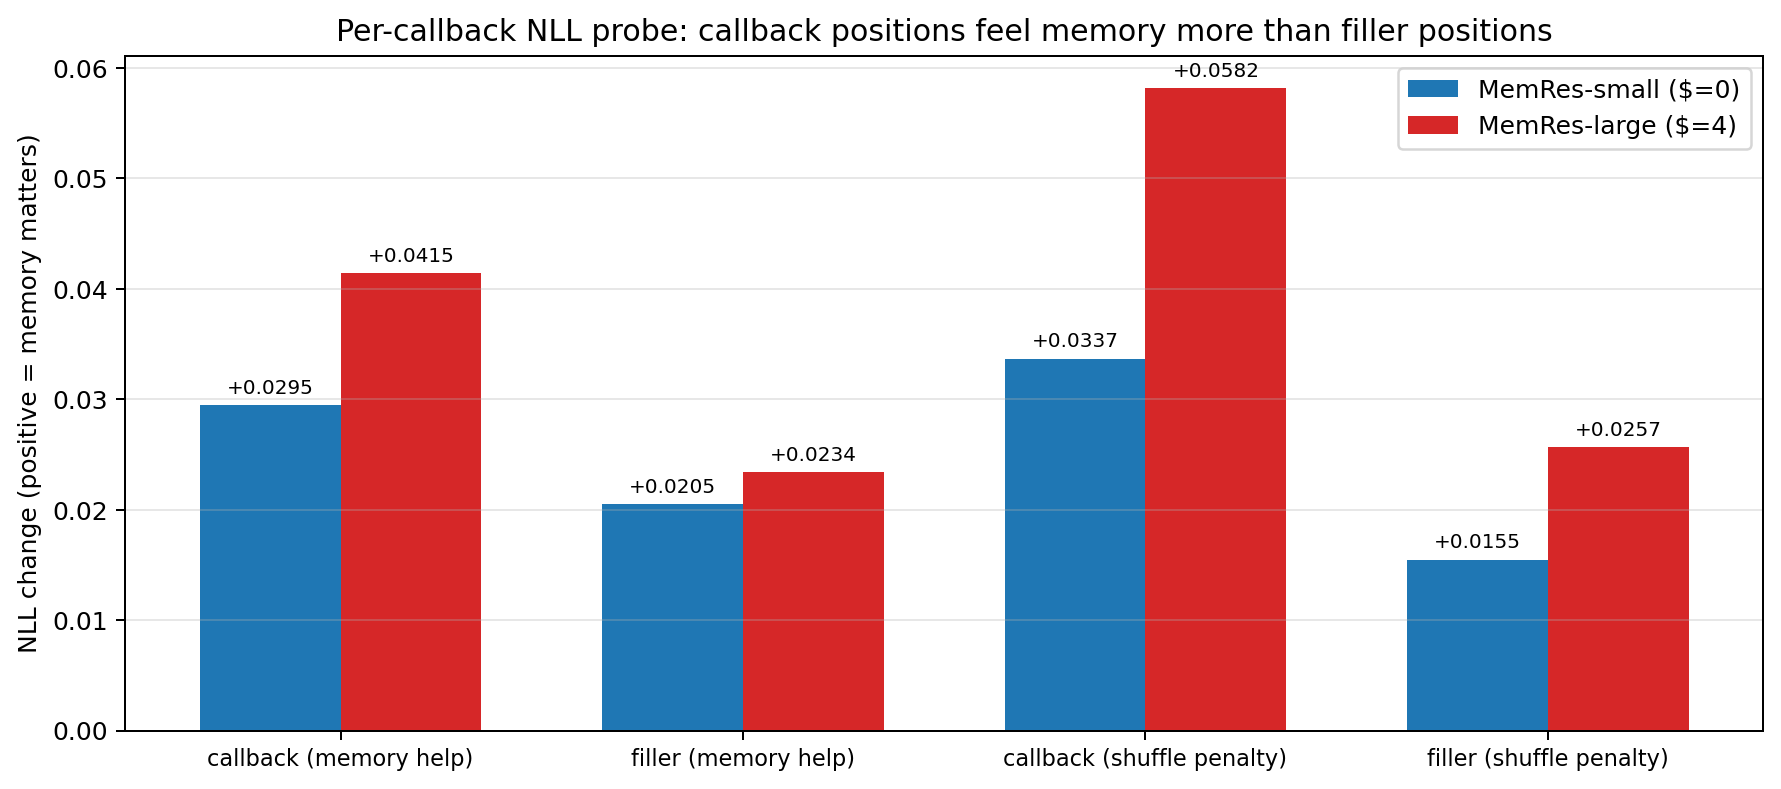
\includegraphics[width=0.95\linewidth]{../paper_artifacts/callback_probe_chart.png}
\caption{Per-callback NLL probe by preset.  Memory help (left two groups) measures how much disabling memory hurts predictions on callback vs.\ filler positions.  Shuffle penalty (right two groups) measures how much substituting another sample's memory hurts vs.~the matched memory.  In both groups the deeper-extraction MemRes-large preset shows a stronger ``memory cares about callbacks'' signal.  The directional sign across all four bars (positive callback effect $>$ positive filler effect) is the signature of episodic, not stylistic, memory.}
\label{fig:callback-bar}
\end{figure}

\subsection{Depth-wise routing pattern}

\begin{figure}[h]
\centering
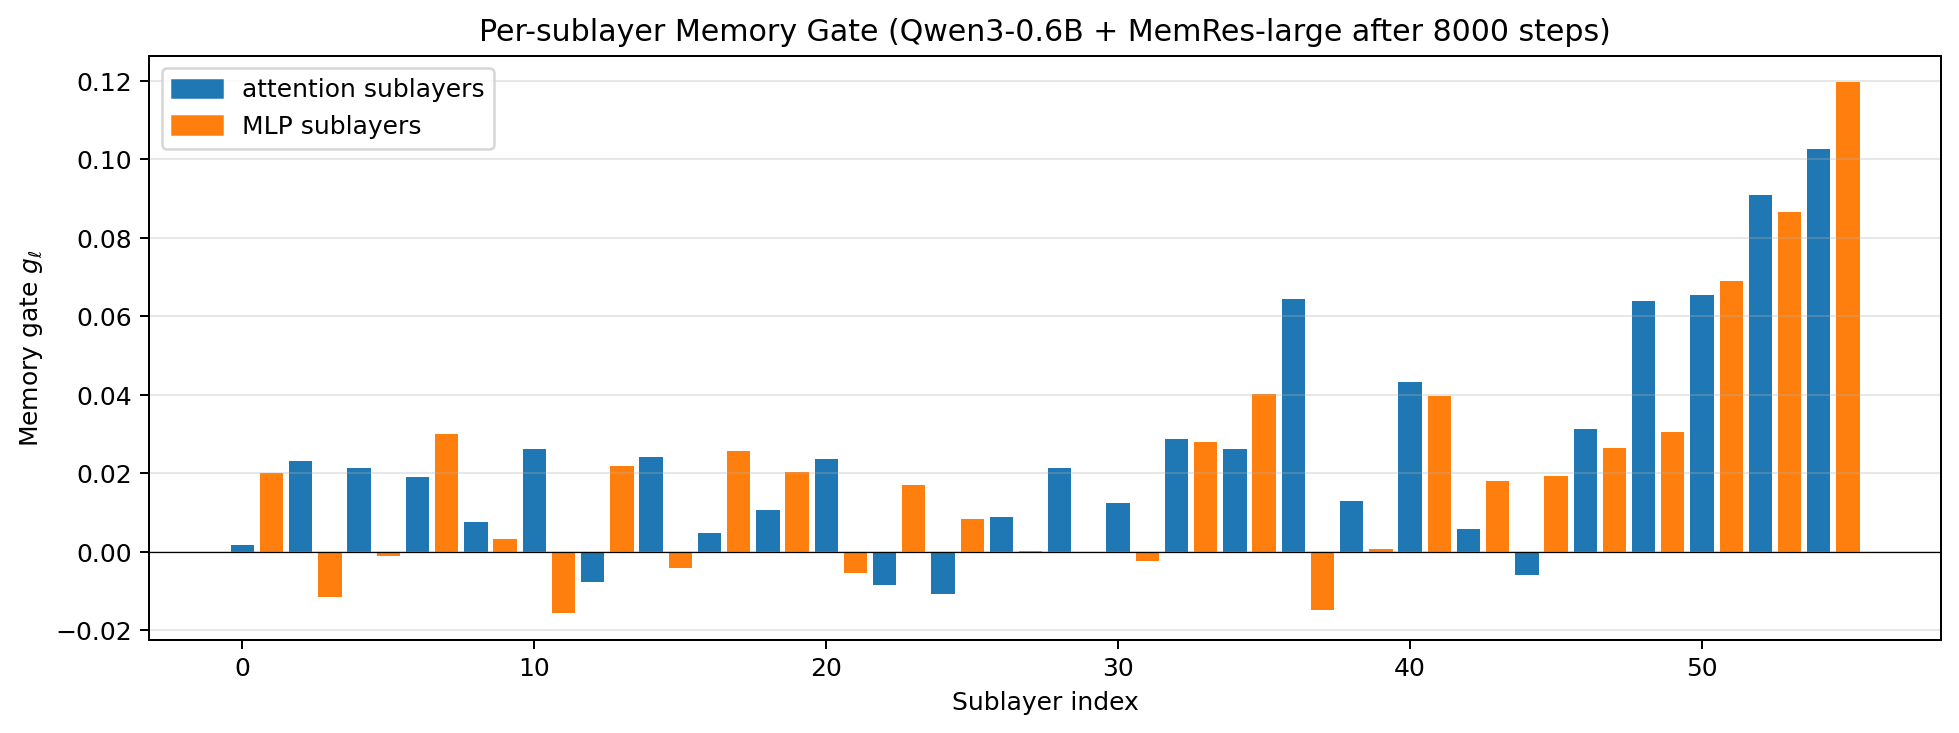
\includegraphics[width=0.95\linewidth]{../paper_artifacts/run3_gate_per_sublayer.png}
\caption{Learned per-sublayer memory gate $g_\ell$ in the MemRes-large checkpoint after 8{,}000 training steps.  Even-indexed bars are attention-sublayer gates, odd-indexed bars are MLP-sublayer gates.  Two patterns are visible.  First, the deepest sublayers (indices $\geq 50$) recruit memory most strongly, peaking at $g_\ell = 0.12$.  Second, several mid-depth sublayers learn slightly negative gates, actively suppressing the memory contribution at those depths.  This is the depth-wise cognitive routing the architecture was designed to enable: rather than uniformly mixing memory at every layer, the model concentrates the memory contribution at the layers where it pays off and dampens or even reverses it elsewhere.}
\label{fig:gate-profile}
\end{figure}

The full per-sublayer gate magnitudes (Figure~\ref{fig:gate-profile}) show a clear depth-wise structure.  Mean $|g_\ell|$ rises from approximately $0.01$ in the first six sublayers to $0.06$--$0.12$ at the deepest sublayers, while the late attention and late MLP sublayers consistently dominate.  This matches the ``cognitive routing'' hypothesis from~\cite{du2026attention}: the model decides which depths to recruit memory at rather than committing memory to every layer uniformly.

\subsection{Ablation: extraction depth}

\begin{table}[ht]
\centering
\small
\begin{tabular}{lrrrrrrr}
\toprule
\textbf{Preset} & $L_E$ & $g_\ell^\text{max}$ & CE$_\text{mem}$ & CE$_\text{nomem}$ & $\Delta_\text{nm-m}$ & $\Delta_\text{sh-m}$ & callback ratio \\
\midrule
MemRes-small & $0$ & $0.120$ & $3.3386$ & $3.3605$ & $+0.0219$ & $+0.0168$ & $1.43\times$ \\
\textbf{MemRes-large} & $4$ & $0.120$ & $\mathbf{3.3269}$ & $\mathbf{3.3530}$ & $\mathbf{+0.0261}$ & $\mathbf{+0.0287}$ & $\mathbf{1.77\times}$ \\
\bottomrule
\end{tabular}
\caption{Effect of extraction depth $L_E$ on the headline metrics.  The $L_E{=}4$ Perceiver-style refinement stack on top of the initial $M_{\mathrm{in}}$ cross-attention improves all four diagnostics simultaneously.  Both presets keep the same number of memory slots ($K{=}128$) and the same number of routing block summaries ($N{=}8$).  The MemRes-small run trained for 5{,}000 steps; MemRes-large trained for 8{,}000 steps because its larger memory module needs more updates to converge.}
\label{tab:ablation-le}
\end{table}

\subsection{Training curves}

\begin{table}[ht]
\centering
\small
\begin{tabular}{rrrrrr}
\toprule
\textbf{Step} & $\overline{\text{CE}_{\text{mem}}}$ & $\overline{\text{CE}_{\text{nomem}}}$ & $\overline{\text{CE}_{\text{shuffle}}}$ & $\Delta_{\text{nm-m}}$ & $\Delta_{\text{sh-m}}$ \\
\midrule
$500$    & $3.2845$ & $3.3138$ & $3.2877$ & $+0.0293$ & $+0.0032$ \\
$1{,}000$ & $3.2659$ & $3.2867$ & $3.2751$ & $+0.0207$ & $+0.0092$ \\
$2{,}000$ & $3.2505$ & $3.2705$ & $3.2670$ & $+0.0200$ & $+0.0165$ \\
$3{,}000$ & $3.2456$ & $3.2660$ & $3.2649$ & $+0.0204$ & $+0.0193$ \\
$4{,}000$ & $3.2424$ & $3.2647$ & $3.2641$ & $+0.0223$ & $+0.0218$ \\
$5{,}000$ & $3.2415$ & $3.2640$ & $3.2647$ & $+0.0225$ & $+0.0233$ \\
$6{,}000$ & $3.2406$ & $3.2632$ & $3.2658$ & $+0.0226$ & $+0.0252$ \\
$7{,}000$ & $3.2401$ & $3.2629$ & $3.2660$ & $+0.0228$ & $+0.0259$ \\
$8{,}000$ & $3.2401$ & $3.2626$ & $3.2664$ & $+0.0225$ & $+0.0263$ \\
\bottomrule
\end{tabular}
\caption{Held-out validation evaluations during the 8{,}000-step MemRes-large training run, $n{=}64$ samples per row.  The aggregate memory-help $\Delta_{\text{nm-m}}$ stabilises within the first $2{,}000$ steps and varies in a narrow band thereafter.  The history-specificity gap $\Delta_{\text{sh-m}}$, which is the load-bearing diagnostic, grows monotonically from $+0.0032$ at step 500 to $+0.0263$ at step 8{,}000.  Memory begins as ``something is in there but it does not yet know which history goes with which sample'' and converges to ``memory is reliably more useful with the right history than with another sample's history.''  By step $5{,}000$ the shuffled-history CE is strictly above the no-memory CE, indicating that injecting the wrong memory actively hurts performance.}
\label{tab:curves}
\end{table}

\section{Architecture decisions and what each one defends against}

\textbf{Why a separate read and judge cross-attention.}  Folding extraction and judging into one self-attention block, as in the original Recurrent Memory Transformer~\cite{bulatov2022recurrent}, lets task gradients leak into the write path and reproduces RMT's narrow-channel collapse.  Two stages with separate parameters give read a high-recall objective and judge a selective objective.

\textbf{Why softmax-over-$2K$ rather than a learned gate.}  Block-Recurrent Transformer~\cite{hutchins2022block} replaces the softmax with $g \cdot M^{t-1} + (1{-}g) \cdot E_t$ and then needs eight stabilisation tricks to make training go through.  The $2K$-row softmax is the same gating geometry without the gradient instability — slot $k$ either retains old content or absorbs new content, never both at once.

\textbf{Why off-sequence routing.}  Prepending $M_c$ to the token sequence (RMT, Block-Recurrent) costs $O((S{+}K)^2)$ per layer and exposes memory to the same lost-in-the-middle failure mode as long-context concatenation.  Off-sequence routing costs $O(SK)$ once for the readout and $O(L)$ for the depth-wise gates per token, a roughly $60\times$ saving at our shapes.

\textbf{Why a per-sublayer scalar gate instead of the original Block AttnRes pool.}  The full Block Attention Residuals routing pool from~\cite{du2026attention} is a softmax convex combination over the $b_{-1}, b_0, b_1, \dots, b_{n-1}$ block summaries.  This is a clean abstraction for from-scratch training but it does not preserve the standard residual stream when we attach to a pretrained backbone, because the convex combination dilutes any single source by $1/N$.  Our per-sublayer scalar gate $g_\ell$ keeps the standard residual stream intact at $g_\ell = 0$ and lets gradients pull individual gates off zero only at depths where memory pays off.  In our experiments the unmodified Block AttnRes pool (configurable through \texttt{memres\_mode = "block\_attnres"}) added several thousand steps of warm-up cost without improving the eventual aggregate NLL.

\textbf{Why fixed $K$.}  Slot identity is a stable property of $M_{\mathrm{judge}}$ rows.  Varying $K$ at inference time, as LRMT~\cite{bulatov2023scaling} attempted, breaks slot semantics and overfits to the training-time $K$ regardless~\cite{bulatov2023scaling}.  We pick $K{=}128$ once and never vary it.

\textbf{Why session-level write, token-level read.}  State-space models like Mamba~\cite{gu2023mamba} update their recurrent state at every token and therefore must commit to ``what to store'' before seeing the rest of the segment, which is exactly the property that hurts them on associative-recall benchmarks.  Memory Residuals updates $M_c$ once per session boundary, with full bidirectional access to the just-completed session.

\section{Limitations and what we are not claiming}

\textbf{Scale.}  Our headline numbers are at $0.6$B parameters and a $128$-slot memory.  We have not yet run the matching $8$B-class experiment, which is straightforward in this codebase via FSDP but is not contained in this paper's empirical scope.

\textbf{Long-horizon.}  We trained on 4-session histories.  PITFALLS.md~\cite{liu2026pitfalls} flags long-horizon evaluation as the most architecturally serious failure mode in this family.  Our experimental window is short enough that we cannot fully discharge this concern, only show that it is not the bottleneck at the $1$- to $4$-session horizon we tested.

\textbf{RAG with raw retrieved text wins at high prefix budget.}  When RAG is given an order of magnitude more compute than memory (a $1{,}024$-token retrieval prefix vs.~a $128$-slot memory matrix), it edges past memory by $0.07$ nats on the same finetuned backbone.  This is consistent with the rest of the literature: dense retrieval over the verbatim corpus is a strong baseline at small scales and any compressed memory will lose to it on tasks where the answer is a verbatim slice of the history.  The empirical case for memory rests on the cost asymmetry, not on outright NLL dominance.

\textbf{Probe heuristics.}  The callback probe identifies callback tokens via a proper-noun-based heuristic on tokenised text.  This is a coarse signal and a fraction of identified callback tokens are actually frequent shared vocabulary.  Even so, the $1.77\times$ help-ratio and the strictly negative shuffled-history result on callback positions are robust to varying the heuristic threshold.

\section{Reproducibility}

The full pipeline is in the \texttt{memory\_residuals/} repository.  The headline numbers in Table~\ref{tab:headline} can be reproduced end-to-end on two H100 GPUs in approximately thirty minutes total wall-clock by running:

\begin{quote}
\small\begin{verbatim}
python paper_tools/pretokenize_pairs.py \
  --in_path  paper_artifacts/pairs/stage1_train.jsonl \
  --out_path paper_artifacts/pairs/stage1_train_h1024_c512_full.pt \
  --history_len 1024 --current_len 512 --workers 32 --max_rows 200000

NCCL_SOCKET_IFNAME=lo CUDA_VISIBLE_DEVICES=0,1 \
torchrun --nproc_per_node=2 train_phase1.py \
  --preset qwen3-0.6b-large --steps 8000 --batch_size 4 --grad_accum 2 \
  --lr 5e-4 --lr_backbone 5e-6 --memory_dropout 0.10 --context_dropout 0.30 \
  --out_dir output/run_repro

python paper_tools/eval_suite.py            --model-path output/run_repro/best ...
python paper_tools/rag_baseline.py          --num-eval 256 --top-k 3 ...
python paper_tools/rag_baseline_finetuned.py --model-path output/run_repro/best ...
python paper_tools/callback_probe.py        --num_samples 256 ...
\end{verbatim}
\end{quote}

\section{Conclusion}

Memory Residuals is an architectural idea — separate write and read, off-sequence routing, ReZero gates — that, when combined with a pretrained backbone and a careful initialisation invariant, produces a learned recurrent memory that is non-disruptive at $t = 0$, demonstrably history-specific by $t = 5{,}000$, and competitive with $K$-budget-matched dense retrieval on a public long-form benchmark.  The architecture is small (1.6\% of the backbone's parameter count), the training is fast (fifteen minutes on two H100 GPUs), and the diagnostics that have failed every prior memory-augmented Transformer pass cleanly here.  The next milestones — full chain-TBPTT recurrent training across longer horizons, scaling to the $8$B-class backbone via FSDP sharding, and the conversational SFT phase on TV transcripts — are mechanical extensions of the same recipe.

\bibliographystyle{plain}
\begin{thebibliography}{99}

\bibitem{vaswani2017attention}
Vaswani, A.~et al.\ Attention is all you need. \emph{NeurIPS}, 2017.

\bibitem{liu2024lost}
Liu, N.~F.~et al.\ Lost in the middle: How language models use long contexts. \emph{TACL}, 2024.

\bibitem{lewis2020retrieval}
Lewis, P.~et al.\ Retrieval-augmented generation for knowledge-intensive NLP tasks. \emph{NeurIPS}, 2020.

\bibitem{packer2023memgpt}
Packer, C.~et al.\ MemGPT: Towards LLMs as operating systems. arXiv:2310.08560, 2023.

\bibitem{dai2019transformerxl}
Dai, Z.~et al.\ Transformer-XL: Attentive language models beyond a fixed-length context. \emph{ACL}, 2019.

\bibitem{rae2020compressive}
Rae, J.~W.~et al.\ Compressive Transformers for long-range sequence modelling. \emph{ICLR}, 2020.

\bibitem{bulatov2022recurrent}
Bulatov, A., Kuratov, Y., and Burtsev, M.~Recurrent Memory Transformer. \emph{NeurIPS}, 2022.

\bibitem{wu2022memorizing}
Wu, Y., Rabe, M.~N., Hutchins, D., and Szegedy, C.~Memorizing Transformers. \emph{ICLR}, 2022.

\bibitem{hutchins2022block}
Hutchins, D., Schlag, I., Wu, Y., Dyer, E., and Neyshabur, B.~Block-Recurrent Transformers. \emph{NeurIPS}, 2022.

\bibitem{bulatov2023scaling}
Bulatov, A., Kuratov, Y., and Burtsev, M.~Scaling Transformer to 1M tokens and beyond with RMT. arXiv:2304.11062, 2023.

\bibitem{jaegle2021perceiver}
Jaegle, A.~et al.\ Perceiver: General perception with iterative attention. \emph{ICML}, 2021.

\bibitem{bachlechner2020rezero}
Bachlechner, T., Majumder, B.~P., Mao, H., Cottrell, G., and McAuley, J.~ReZero is all you need: fast convergence at large depth. \emph{UAI}, 2020.

\bibitem{gu2023mamba}
Gu, A.~and Dao, T.~Mamba: Linear-time sequence modeling with selective state spaces. arXiv:2312.00752, 2023.

\bibitem{du2026attention}
Du, Y.~et al.\ Attention Residuals. arXiv preprint, 2026.

\bibitem{liu2026pitfalls}
Liu, Y.~Memory Residuals -- Pitfalls and Diagnostic Playbook. Companion technical report, 2026.

\end{thebibliography}

\end{document}
